\documentclass[tikz,border=6pt]{standalone}
\usepackage{amsmath,amssymb,mathtools,physics,bm,nicefrac,wasysym}
\usepackage{xcolor}

\definecolor{colone}{RGB}{180,60,60}
\definecolor{coltwo}{RGB}{60,110,180}
\definecolor{colthree}{RGB}{60,140,80}

\definecolor{accent}{HTML}{A13D2C}
\definecolor{accent2}{HTML}{2B5F6B}
\definecolor{muted}{HTML}{5A564F}
\definecolor{panel}{HTML}{F8F6F0}
\definecolor{linecol}{HTML}{D8D2C4}
\definecolor{ink}{HTML}{1E1C1A}
\definecolor{astroblue}{HTML}{1B4F72}
\definecolor{astrodark}{HTML}{17202A}
\definecolor{sunyellow}{HTML}{E8A33D}

\usetikzlibrary{calc,arrows.meta,positioning,decorations.pathreplacing,decorations.markings,angles,quotes,shapes.geometric}
\usepackage{tikz-3dplot}

\newcommand{\vecr}{\vec r}
\newcommand{\vecL}{\vec L}
\newcommand{\vecA}{\vec A}
\newcommand{\vecf}{\vec f}
\newcommand{\vecF}{\vec F}
\newcommand{\vecp}{\vec p}
\newcommand{\avg}[1]{\left\langle #1\right\rangle}
\newcommand{\vecx}{\vec x}
\newcommand{\hatn}{\hat n}
\newcommand{\rhat}{\hat r}
\newcommand{\phihat}{\hat\phi}
\newcommand{\thetahat}{\hat\theta}
\newcommand{\note}[1]{\textcolor{blue!60!black}{\textit{[#1]}}}

\newcommand{\LST}{\mathrm{LST}}
\newcommand{\GST}{\mathrm{GST}}
\newcommand{\GMST}{\mathrm{GMST}}
\newcommand{\GAST}{\mathrm{GAST}}
\newcommand{\LMST}{\mathrm{LMST}}
\newcommand{\LAST}{\mathrm{LAST}}
\newcommand{\UT}{\mathrm{UT}}
\newcommand{\UTC}{\mathrm{UTC}}
\newcommand{\TAI}{\mathrm{TAI}}
\newcommand{\TT}{\mathrm{TT}}
\newcommand{\TDB}{\mathrm{TDB}}
\newcommand{\JD}{\mathrm{JD}}
\newcommand{\MJD}{\mathrm{MJD}}
\newcommand{\EoT}{\mathrm{EoT}}
\newcommand{\SNR}{\mathrm{SNR}}
\newcommand{\RON}{\mathrm{RON}}



\begin{document}
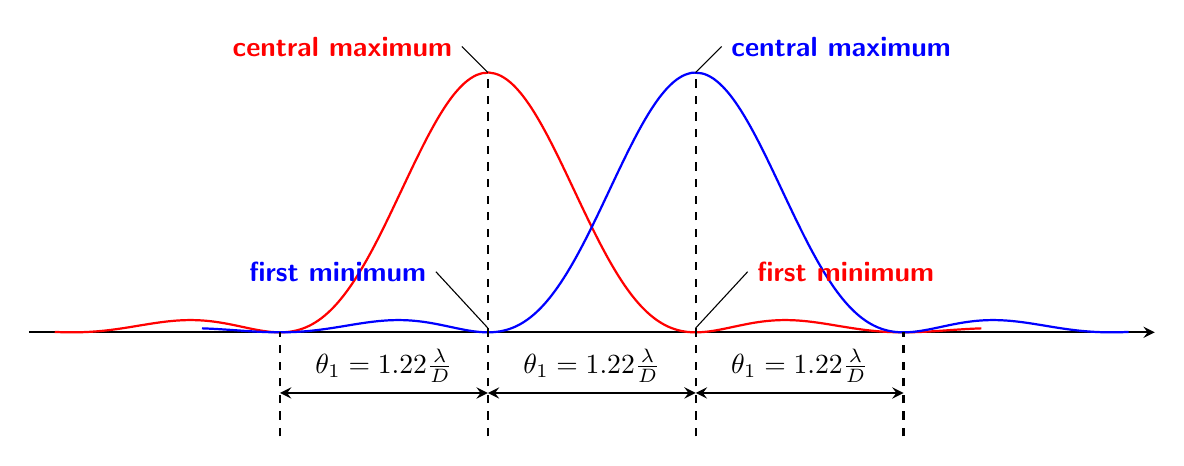
\begin{tikzpicture}[
    scale=1.1,
    >=stealth,
    declare function={
        sinc(\x) = (\x==0 ? 1 : sin(deg(\x))/\x);
    }
]
    \def\xR{-1.2}
    \def\xB{1.2}
    \def\dx{2.4} 

    \draw[->, thick] (-6.5,0) -- (6.5,0);

    \draw[red, thick, domain=-6.2:4.5, samples=300, smooth] 
        plot (\x, {3.0 * pow(sinc(3.14159 * (\x - \xR) / \dx), 2)});

    \draw[blue, thick, domain=-4.5:6.2, samples=300, smooth] 
        plot (\x, {3.0 * pow(sinc(3.14159 * (\x - \xB) / \dx), 2)});

    \draw[dashed, thick] (\xR, -1.2) -- (\xR, 3.0);
    \draw[dashed, thick] (\xB, -1.2) -- (\xB, 3.0);
    \draw[dashed, thick] ({\xR - \dx}, -1.2) -- ({\xR - \dx}, 0);
    \draw[dashed, thick] ({\xB + \dx}, -1.2) -- ({\xB + \dx}, 0);

    \draw[<->, thick] ({\xR - \dx}, -0.7) -- node[above] {$\theta_1 = 1.22 \frac{\lambda}{D}$} (\xR, -0.7);
    \draw[<->, thick] (\xR, -0.7) -- node[above] {$\theta_1 = 1.22 \frac{\lambda}{D}$} (\xB, -0.7);
    \draw[<->, thick] (\xB, -0.7) -- node[above] {$\theta_1 = 1.22 \frac{\lambda}{D}$} ({\xB + \dx}, -0.7);

    \draw[thin] (-1.5, 3.3) -- (\xR, 3.0);
    \node[red, font=\bfseries\sffamily, left] at (-1.5, 3.3) {central maximum};

    \draw[thin] (1.5, 3.3) -- (\xB, 3.0);
    \node[blue, font=\bfseries\sffamily, right] at (1.5, 3.3) {central maximum};

    \draw[thin] (-1.8, 0.7) -- (\xR, 0.05);
    \node[blue, font=\bfseries\sffamily, left] at (-1.8, 0.7) {first minimum};

    \draw[thin] (1.8, 0.7) -- (\xB, 0.05);
    \node[red, font=\bfseries\sffamily, right] at (1.8, 0.7) {first minimum};
    \end{tikzpicture}
\end{document}
